\documentclass[conference]{IEEEtran}
\IEEEoverridecommandlockouts
\usepackage{blindtext}
\usepackage{amsmath}
\usepackage{gensymb}
\usepackage{graphicx}
\graphicspath{ {./images/}  }

\begin{document}

\title{ECSE 331\\
    Laboratory No. 3\\
    MOSFET DC Characteristics in PSPICE\\
    \Large \today\\
}

\author
{
    \IEEEauthorblockN{Seyed Yazdan Zinati}
    \IEEEauthorblockA{260928077 \\
    \textit{seyed.zinati@mail.mcgill.ca}}

    \and

    \IEEEauthorblockN{James Wu}
    \IEEEauthorblockA{260929944 \\
    \textit{james.wu4@mail.mcgill.ca}}
}
\maketitle
\clearpage

\begin{abstract}
    A MOSFET is a three-terminal device that allows current to flow through it when a certain threshold voltage is reached. The three terminals of a MOSFET are called the gate, the source, and the drain. There are two types of MOSFETs: NMOS FET and PMOS FET. Current flows from the drain to the source for NMOS FET and vice versa for PMOS FET. For NMOS FET, current will not flow through the device unless the voltage across the gate terminals and the source terminal $V_{GS}$ is greater than a certain threshold voltage $V_{t}$. For PMOS FET, current will not flow through the device unless $V_{GS}$ is less than $V_{t}$.  MOSFETs have two modes of operation: triode and saturation. The difference between these two modes is that the equation to calculate the current flowing through the MOSFET $I_{D}$ is different. In triode mode, $I_{D}$ increases much more rapidly, as the voltage across the drain and source increases $V_{DS}$, than in saturation mode. NMOS FETs operate in triode mode when $V_{DS} < V_{GS} - V_{t}$ , and they operate in saturation mode when $V{DS} > V_{GS} - V_{t}$.  For PMOS FETs, the conditions of the operation modes are the opposite of NMOS FET; triode mode when $V_{DS} > V_{GS} - V_{t}$ and saturation mode when $V_{DS} < V_{GS} - V_{t}$.

\end{abstract}

\section{Introduction}
MOSFETs are three-terminal devices that allows current to flow through it when $V_{GS}$ is either greater than or less than $V_{t}$. The operating mode of the MOSFET depends on $V_{DS}$ compared to $V_{GS} - V_{t}$.

In this laboratory, we conduct experiments on a circuit that has an NMOS FET using circuit simulation software. PSPICE software is used to build and simulate circuits. The circuit that will be built using PSPICE is shown in Figure 1. We first examine the $I_{D}-V_{DS}$ characteristics of the MOSFET. Then, we determine the MOSFET transconductance. Finally, we examine the effects of temperature on MOSFET.\\

\begin{figure}[h]
    \centering
    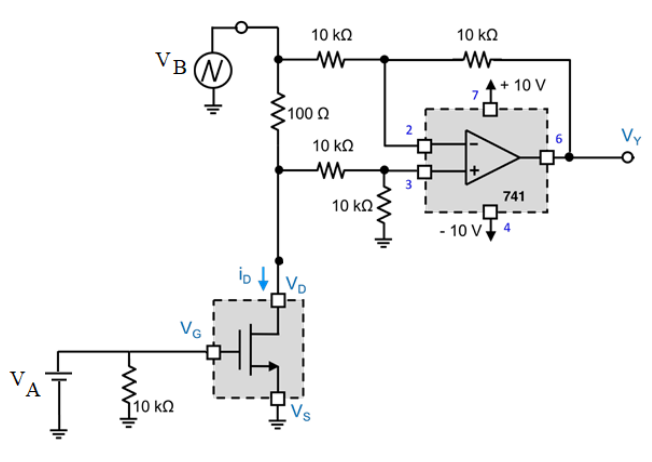
\includegraphics[scale=0.4]{Schematic}
    \caption{Setup for measuring MOSFET $I-V$ characteristics}
\end{figure}

\subsection{Task 1}
The first part of the lab involves measuring NMOS FET characteristics. First, we plot $V_{DS}$ vs time and $I_{D}$ vs time. It should be observed that $I_D$ remains zero despite any change in $V_{DS}$. We then determine the threshold voltage of the NMOS FET by increasing $V_{GS}$ until $I_D$ exceeds 0.5mA.

Next, we plot the voltage output ($V_Y$) of the op-amp divided by 100 vs time and the current through the $100 \Omega $ resistance vs time. These two plots are then compared with each other and examined.

Finally, we increase $V_{GS}$ in increments of 1V until $V_{GS}$ reaches 5V while plotting $I_D$ vs $V_{DS}$ for each value of $V_{GS}$. From the plot of $I_D$ vs $V_{DS}$ for each $V_{GS}$ value, we can obtain the early voltage of the MOSFET. This can be done by extending the linear trends of the saturation modes of the traces to the left until they reach $I_D = 0$. The corresponding $V_{DS}$ value is the negative value of the early effective voltage.

\subsection{Task 2}
The second part of the lab involves the computation of the MOSFET transconductance ($g_m$) of the NMOS FET. The transconductance is found using the following equation:


\[g_m = \frac{\Delta i_D}{v_{GS}}\]


The circuit must first be modified by replacing the saw-tooth signal $V_B$ with a DC voltage source set to 5V and $V_A$ needs to be set to 3V. $I_D$ and $V_GS$ is recorded at these values and they’re recorded again when $V_A$ is adjusted by 0.1V. $\Delta I_D$ and $\Delta V_{GS}$ are then found by taking the differences between the measured $V_{GS}$ and $I_D$ and the transconductance is computed.

\subsection{Task 3}
The third part of the lab examines the effect of temperature on the MOSFET. First, the circuit must be restored back to its original state in Figure1 by using the saw-tooth waveform as $V_B$ and setting $V_A$ to 3V. The simulation is conducted at temperatures 10°C, 20°C, 27°C, 35°C and 50°C. The $I_D$ vs $V_{DS}$ plots at these temperatures are compared.
\section{Analysis}


\section{Conclusion}

\section{Appendix}
\end{document}
